A square table of size $7\times 7$ with the four corner squares deleted is given.
\begin{itemize}
	\item What is the smallest number of squares which need to be colored black so that a $5-$square entirely uncolored Greek cross (see Figure) cannot be found on the table?
	\item Prove that it is possible to write integers in each square in a way that the sum of the integers in each Greek cross is negative while the sum of all integers in the square table is positive.
\end{itemize}
\begin{center}
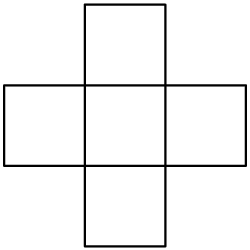
\includegraphics[width = 25.0mm]{img/fig0.png}
\end{center}
